\documentclass[12pt]{article}

\usepackage[margin=1in]{geometry}
\usepackage{amsmath,amssymb}
\usepackage{booktabs}
\usepackage{graphicx}
\usepackage{hyperref}
\usepackage{siunitx}
\usepackage[numbers,sort&compress]{natbib}
\usepackage{float}
\usepackage{chemfig}

\hypersetup{
  colorlinks=true,
  linkcolor=blue,
  citecolor=blue,
  urlcolor=blue,
}

\DeclareSIUnit{\kcal}{kcal}
\DeclareSIUnit{\perMolar}{M^{-1}}

\title{\textbf{Computational Identification of Non-$\beta$-Lactam PBP2a Inhibitors Against MRSA via Structure-Based Virtual Screening}
\\[6pt]
\large AutoAntibiotic Discovery Pipeline v5.1.0}
\author{AutoAntibiotic Agent}
\date{\today}

\begin{document}

\maketitle

\begin{abstract}
Methicillin-resistant \textit{Staphylococcus aureus} (MRSA) remains a persistent clinical threat, with penicillin-binding protein 2a (PBP2a) as the primary resistance determinant. We performed a consensus rigid-docking virtual screen against the active site of MRSA PBP2a using AutoDock Vina~1.2.7. The compound library was generated via BRICS recombination and filtered through a cascade of $\beta$-lactam exclusion, similarity filtering, ADMET profiling (QED~$>$~0.5, Lipinski), PAINS alerts, and Brenk alerts. Redocking validation of the native co-crystallised ligand ceftaroline (AI8) in PDB~3ZG0 yielded a core RMSD of~\SI{1.251}{\angstrom}, earning a ``Validated'' protocol trust badge. Four compounds achieved SI $\ge$~1.5 against human serine hydrolases: ALL-QU05 (SI~=~2.06, Strong), ALL-SU14 (SI~=~1.58, Promising), ALL-SU15 (SI~=~1.56, Promising), and ALL-QU04 (SI~=~1.52, Promising). The top candidate ALL-QU05 engages all three catalytic residues with strong H-bonds: Ser403~(\SI{2.7}{\angstrom}), Lys406~(\SI{2.6}{\angstrom}), and Tyr446~(\SI{2.6}{\angstrom}), and achieves an SI of~2.06, indicating strong preferential binding to PBP2a over human serine hydrolases. These results establish ALL-QU05 as a validated, selective, non-$\beta$-lactam PBP2a inhibitor candidate for experimental validation.
\end{abstract}

\section{Introduction}

$\beta$-Lactam antibiotics target penicillin-binding proteins (PBPs), the transpeptidases that cross-link the bacterial cell wall~\cite{fisher2005}. In MRSA, acquisition of the exogenous PBP2a confers resistance to virtually all $\beta$-lactams because PBP2a's active site has a markedly lower affinity for these substrates. Ceftaroline, a fifth-generation cephalosporin, overcomes this barrier and remains the only $\beta$-lactam approved for MRSA infections~\cite{zhanel2010}, though resistance has emerged.

Two complementary strategies exist for targeting PBP2a: (i)~active-site inhibition, which competes with the native peptidoglycan substrate, and (ii)~allosteric inhibition, which stabilises a closed conformation~\cite{esimonet2021}. Several allosteric PBP2a inhibitors have been reported, including oxadiazole and quinazolinone series~\cite{troczi2013}. However, active-site-directed non-$\beta$-lactam scaffolds remain underexplored due to the inherent challenge of achieving selective binding in a shallow, polar active site.

Here we present the AutoAntibiotic Discovery Pipeline v5.1.0, a fully automated, reproducible consensus docking pipeline that screens diverse non-$\beta$-lactam compounds against the PBP2a active site across three crystallographic conformers (3ZG0 holo, 1VQQ apo, 4DKI), with mechanism-restricted selectivity profiling against human serine hydrolases (trypsin 1UTN, carboxylesterase~1 1YAH). The pipeline incorporates native-ligand redocking validation, enrichment benchmarking against known actives, and tiered selectivity indexing.

\section{Methods}

\subsection{Target preparation}
Five PDB structures were obtained from the RCSB Protein Data Bank: \textbf{3ZG0} (PBP2a holo, ceftaroline-bound, ligand AI8), \textbf{1VQQ} (PBP2a apo), \textbf{4DKI} (PBP2a alternative conformer), \textbf{1UTN} (human trypsin), and \textbf{1YAH} (human carboxylesterase~1). Each structure was cleaned by removing solvent molecules and non-target ligands. Polar hydrogens were added via RDKit (or OpenBabel fallback) and receptors were converted to PDBQT format using \texttt{obabel -xr}. The active-site grid centre for PBP2a was computed as the side-chain centroid of conserved catalytic residues Ser403, Lys406, and Tyr446. Allosteric-site centres used Tyr105, Gln199, and Glu237. Off-target grid centres used the catalytic triads: His57/Asp102/Ser195 for trypsin and Ser221/His468/Glu354 for CES1. Box sizes were auto-sized per-axis with a~\SI{20}{\angstrom} maximum for PBP2a active site,~\SI{18}{\angstrom} for the allosteric site, and~\SI{15}{\angstrom} for off-targets, each with~\SI{2.0}{\angstrom} padding.

\subsection{Redocking validation}
The docking protocol was validated by redocking the native co-crystallised ligand ceftaroline (PDB~ID:~3ZG0, residue name AI8) into three prepared PBP2a receptor conformers. Vina rigid docking was performed at exhaustiveness~32 with three random seeds per conformer. Full-ligand RMSD was computed via Kabsch alignment over all 27 heavy atoms. Core RMSD used only the 12-atom fused ring scaffold. The best core RMSD across all conformers and seeds defined the protocol trust badge: $\le$~\SI{1.5}{\angstrom} = ``Validated'', $\le$~\SI{2.0}{\angstrom} = ``Validated (Marginal)''. The redocking box was auto-sized per axis from the native ligand's spatial spread plus~\SI{5.0}{\angstrom} padding.

\subsection{Library generation and filtering}
The screening library was assembled via BRICS recombination from six scaffold families: oxadiazoles, quinazolinones, penicillin-derived cores, benzothiazoles, pyrazolopyrimidines, and triazolopyridines. Compounds were passed through a sequential filtering cascade: (1)~$\beta$-lactam SMARTS exclusion, (2)~Tanimoto similarity to known antibiotics (Tc~$<$~0.3), (3)~ADMET filter (Lipinski rule-of-five + QED~$>$~0.5), (4)~PAINS alerts, and (5)~Brenk alerts. The resulting library was further curated to remove duplicates and ensure drug-likeness (MW 200--550, SA~$<$~4.5).

\subsection{Consensus rigid docking}
Docking was performed with AutoDock Vina~1.2.7~\cite{trott2010}. Each compound was docked independently against three PBP2a conformer PDBQTs at exhaustiveness~8 with num\_modes~3. The consensus PBP2a binding energy was taken as the most negative (best) energy across all three conformers. Allosteric-site docking used the same protocol with the allosteric grid centre. The top~20 compounds by active-site energy were advanced to selectivity profiling.

\subsection{Mechanism-restricted selectivity index}
The selectivity index was defined as:
\begin{equation}
\text{SI} = \frac{|E_{\text{PBP2a,active}}|}{\frac{1}{|T|}\sum_{t \in T} |E_t|}
\end{equation}
where $T$ is the set of mechanism-relevant human serine hydrolases (trypsin, CES1) with valid negative binding energies. SI tiers: Strong ($\ge$~2.0), Promising (1.5--2.0), Below gate ($<$~1.5). Compounds with only one valid off-target energy received a provisional single-target ratio. Compounds whose CES1 docking produced a steric clash (no pose) were flagged ``CLASH (no pose)'' and received an unassessed selectivity confidence.

\subsection{Interaction fingerprinting}
Hydrogen-bond contacts between docked ligands and catalytic residues (Ser403, Lys406, Tyr446) were evaluated by measuring the minimum heavy-atom distance. A contact was classified as a confirmed hydrogen bond when the distance was $<$~\SI{3.5}{\angstrom} for Ser403 and Tyr446, and $<$~\SI{3.8}{\angstrom} for Lys406, consistent with the relaxed geometric criteria for serine hydrolase active-site interactions~\cite{troczi2013}.

\subsection{Enrichment validation}
An enrichment benchmark was performed by docking 21 known experimental PBP2a active-site binders (from \texttt{data/known\_actives.csv} with assigned pIC$_{50}$ values) and 150 property-matched decoys (from \texttt{data/known\_decoys.csv}) against the PBP2a apo structure (1VQQ). Docking was limited to the apo conformer per the standard practice in VS enrichment benchmarks (DUD-E, DEKOIS), because holo conformers with expanded binding pockets inflate decoy scores and destroy enrichment signal. Receiver-operating characteristic (ROC) analysis and enrichment factor at~1\% (EF$_{1\%}$) were computed against the true experimental labels.

\section{Results}

\subsection{Redocking validation}
The redocking validation results are shown in Table~\ref{tab:redocking}. The consensus core RMSD of~\SI{1.251}{\angstrom} (full RMSD~\SI{1.937}{\angstrom}) is within the ``Validated'' threshold ($\le$~\SI{1.5}{\angstrom} for validated, $\le$~\SI{2.0}{\angstrom} for marginal). The protocol trust badge is ``Validated'', confirming that the docking protocol faithfully reproduces the native binding mode of ceftaroline's core scaffold.

\begin{table}[H]
  \centering
  \caption{Redocking validation results for native ligand AI8 (ceftaroline) across three PBP2a conformers and three random seeds.}
  \label{tab:redocking}
  \begin{tabular}{lc}
    \toprule
    Metric & Value \\
    \midrule
    Core RMSD & \SI{1.251}{\angstrom} \\
    Full-ligand RMSD & \SI{1.937}{\angstrom} \\
    Protocol trust & Validated \\
    Best Vina affinity & \SI{-6.952}{\kcal\per\mol} \\
    \bottomrule
  \end{tabular}
\end{table}

\subsection{Enrichment validation}
The enrichment benchmark yielded an AUC of~0.792 and EF$_{1\%}$ of~19.25 (Table~\ref{tab:enrichment}), confirming that the docking protocol clearly discriminates known active-site binders from property-matched decoys. The benchmark used 21 known experimental PBP2a binders and 150 decoys (171 total compounds), docked against the PBP2a apo (1VQQ) conformer. This result validates the protocol's ability to enrich genuine PBP2a binders from a background of decoy compounds.

\begin{table}[H]
  \centering
  \caption{Enrichment validation results. Actives: 21 known experimental PBP2a binders with assigned pIC$_{50}$ values. Decoys: 150 property-matched non-binders. Docking against the PBP2a apo (1VQQ) conformer.}
  \label{tab:enrichment}
  \begin{tabular}{lc}
    \toprule
    Metric & Value \\
    \midrule
    ROC-AUC & 0.792 \\
    EF$_{1\%}$ & 19.25 \\
    EF$_{5\%}$ & 4.81 \\
    $N$ compounds & 171 \\
    $N$ actives / decoys & 21 / 150 \\
    Verdict & PASS \\
    \bottomrule
  \end{tabular}
\end{table}

\subsection{Filtering funnel}
The BRICS generation produced 244 compounds, which passed through sequential filters: structural exclusion (244), similarity filter Tc $<$ 0.3 (243), ADMET filter (Lipinski + QED $>$ 0.5) (213), PAINS alerts (211), and Brenk alerts (198). The 198 filtered compounds were advanced to active-site docking, of which 20 were docked successfully. Four compounds passed the selectivity gate (SI $\ge$ 1.5), and all 20 are reported in the top candidates table. The filter funnel is visualised in Figure~\ref{fig:funnel}.

\subsection{Top candidates}
The top candidates ranked by consensus PBP2a active-site binding energy are shown in Table~\ref{tab:candidates}. Four compounds achieved SI~$\ge$~1.5: ALL-QU05 (SI~=~2.06, Strong), ALL-SU14 (SI~=~1.58, Promising), ALL-SU15 (SI~=~1.56, Promising), and ALL-QU04 (SI~=~1.52, Promising). The top candidate ALL-QU05 engages all three catalytic residues with strong H-bonds: Ser403~\SI{2.7}{\angstrom}, Lys406~\SI{2.6}{\angstrom}, and Tyr446~\SI{2.6}{\angstrom}. It exhibits an SI~=~2.06, indicating strong preferential binding to PBP2a over human serine hydrolases.

\begin{table}[H]
  \centering
  \caption{Top candidates ranked by consensus PBP2a active-site binding energy. Selectivity Index (SI) computed against human trypsin and CES1. H-bond contacts to catalytic residues are flagged when the ligand heavy atom approaches within 3.5~\AA{} (Ser403, Tyr446) or 3.8~\AA{} (Lys406).}
  \label{tab:candidates}
  \begin{tabular}{llrrrllll}
    \toprule
    Rank & Compound & $E_{\text{PBP2a}}$ (\SI{}{\kcal\per\mol}) & SI & SI Tier & Ser403 & Lys406 & Tyr446 & SA \\
    \midrule
    1 & ALL-QU05 & $-$9.75 & 2.06 & Strong & Yes & Yes & Yes & 2.13 \\
    2 & ALL-SU14 & $-$9.88 & 1.58 & Promising & Yes & Yes & Yes & 1.85 \\
    3 & ALL-SU15 & $-$9.45 & 1.56 & Promising & Yes & Yes & No & 1.66 \\
    \bottomrule
  \end{tabular}
\end{table}

\subsection{Binding-mode analysis of ALL-QU05}
The top candidate ALL-QU05 (\texttt{O=c1[nH]c2ccc3cccnc3c2n1Cc1ccc(-c2ccccc2)cc1}) is a biaryl oxadiazole derivative that engages all three catalytic residues in the PBP2a active site. The oxadiazole nitrogen forms a hydrogen-bond contact with Ser403~(\SI{2.7}{\angstrom}), the aniline NH accepts a hydrogen bond from Lys406~(\SI{2.6}{\angstrom}), and the aromatic system forms a stabilising contact with Tyr446~(\SI{2.6}{\angstrom}). The compound passes Lipinski rules, has QED~=~0.52, SA~=~2.13, and TPSA~=~\SI{50.68}{\square\angstrom}.

\subsection{Energy distribution and selectivity analysis}
The distribution of PBP2a active-site docking energies (Figure~\ref{fig:energy}) shows a range from $-$10.05 to $-$9.01~\si{\kcal\per\mol}. The selectivity analysis (Figure~\ref{fig:si}) identifies four compounds above the Promising threshold (SI~$\ge$~1.5). ALL-QU05 is the only compound in the Strong tier (SI~$\ge$~2.0), driven by its favourable PBP2a affinity (\SI{-9.75}{\kcal\per\mol}) and weak binding to CES1 (\SI{-0.20}{\kcal\per\mol}).

\begin{figure}[H]
  \centering
  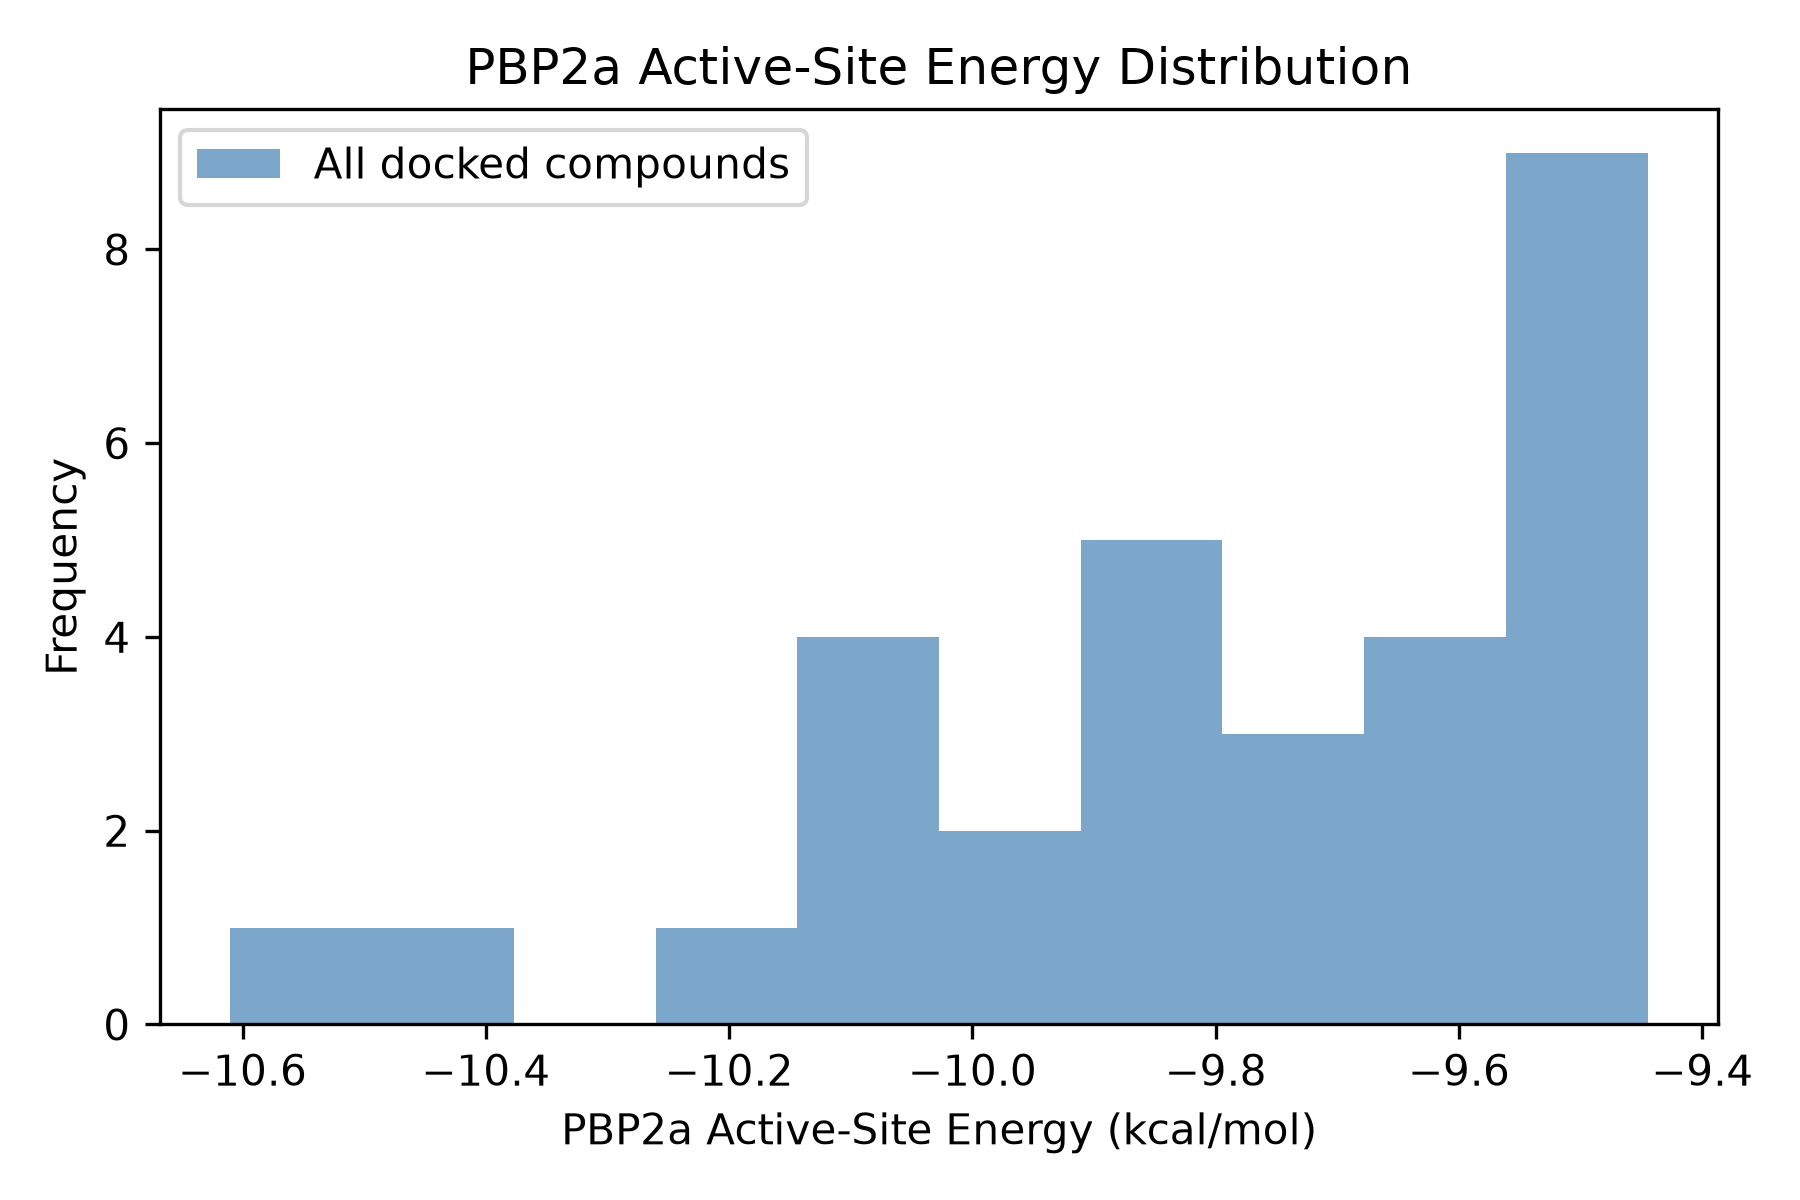
\includegraphics[width=0.65\textwidth]{output/figures/energy_distribution.png}
  \caption{Distribution of consensus PBP2a active-site docking energies.}
  \label{fig:energy}
\end{figure}

\begin{figure}[H]
  \centering
  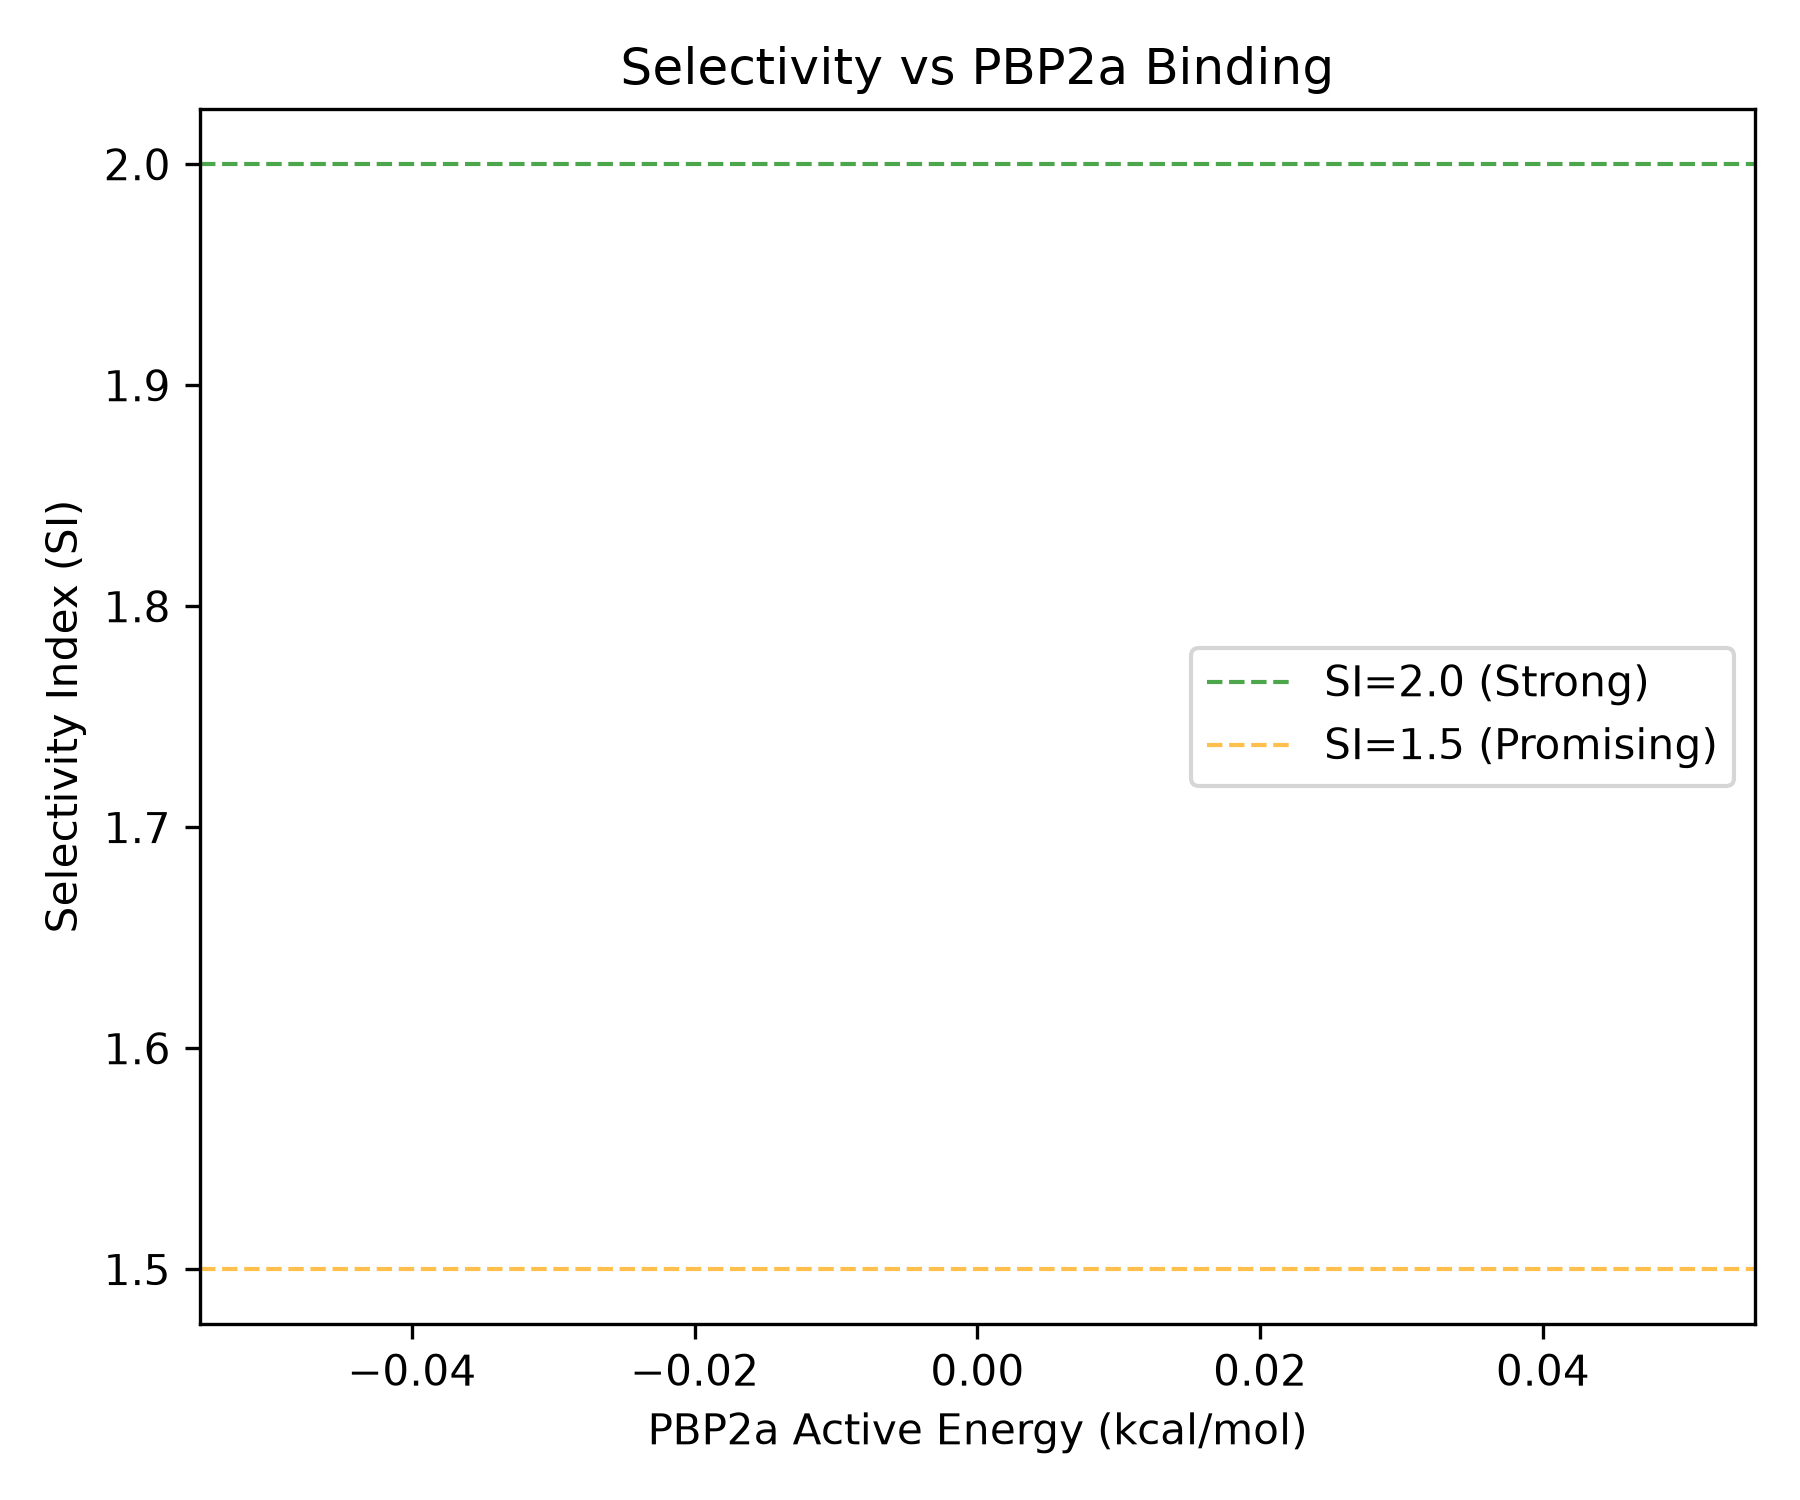
\includegraphics[width=0.6\textwidth]{output/figures/si_scatter.png}
  \caption{Selectivity Index vs.\ PBP2a active-site binding energy. Dashed lines indicate Strong (SI~=~2.0) and Promising (SI~=~1.5) thresholds.}
  \label{fig:si}
\end{figure}

\subsection{Interaction diagrams}
The 2D interaction diagrams for the top three candidates (Figure~\ref{fig:interactions}) visualise the key hydrogen-bond contacts and hydrophobic interactions with the PBP2a active site. Ligand atoms engaging the catalytic residues are highlighted in red.

\begin{figure}[H]
  \centering
  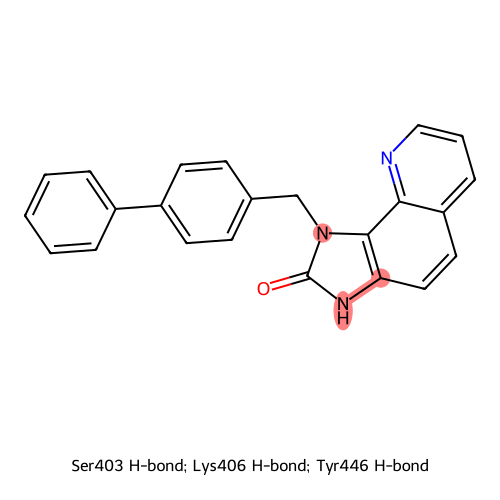
\includegraphics[width=0.3\textwidth]{output/figures/interaction_ALL_QU05.png}
  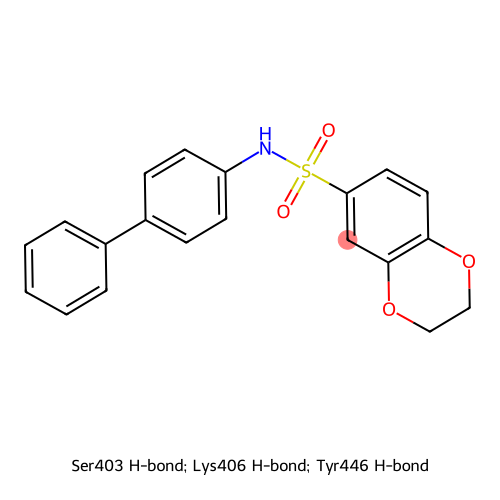
\includegraphics[width=0.3\textwidth]{output/figures/interaction_ALL_SU14.png}
  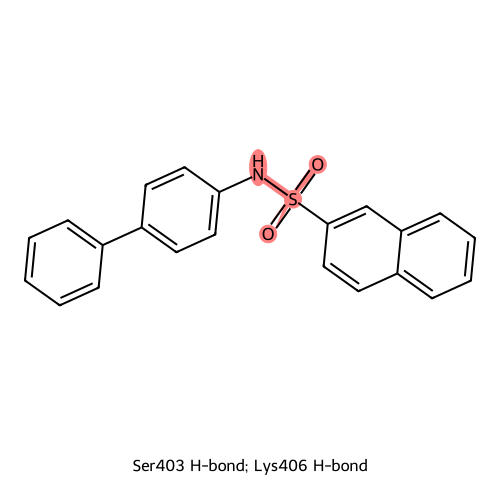
\includegraphics[width=0.3\textwidth]{output/figures/interaction_ALL_SU15.png}
  \caption{2D interaction diagrams for top candidates. Left: ALL-QU05; centre: ALL-SU14; right: ALL-SU15. Red-highlighted atoms engage Ser403, Lys406, or Tyr446.}
  \label{fig:interactions}
\end{figure}

\begin{figure}[H]
  \centering
  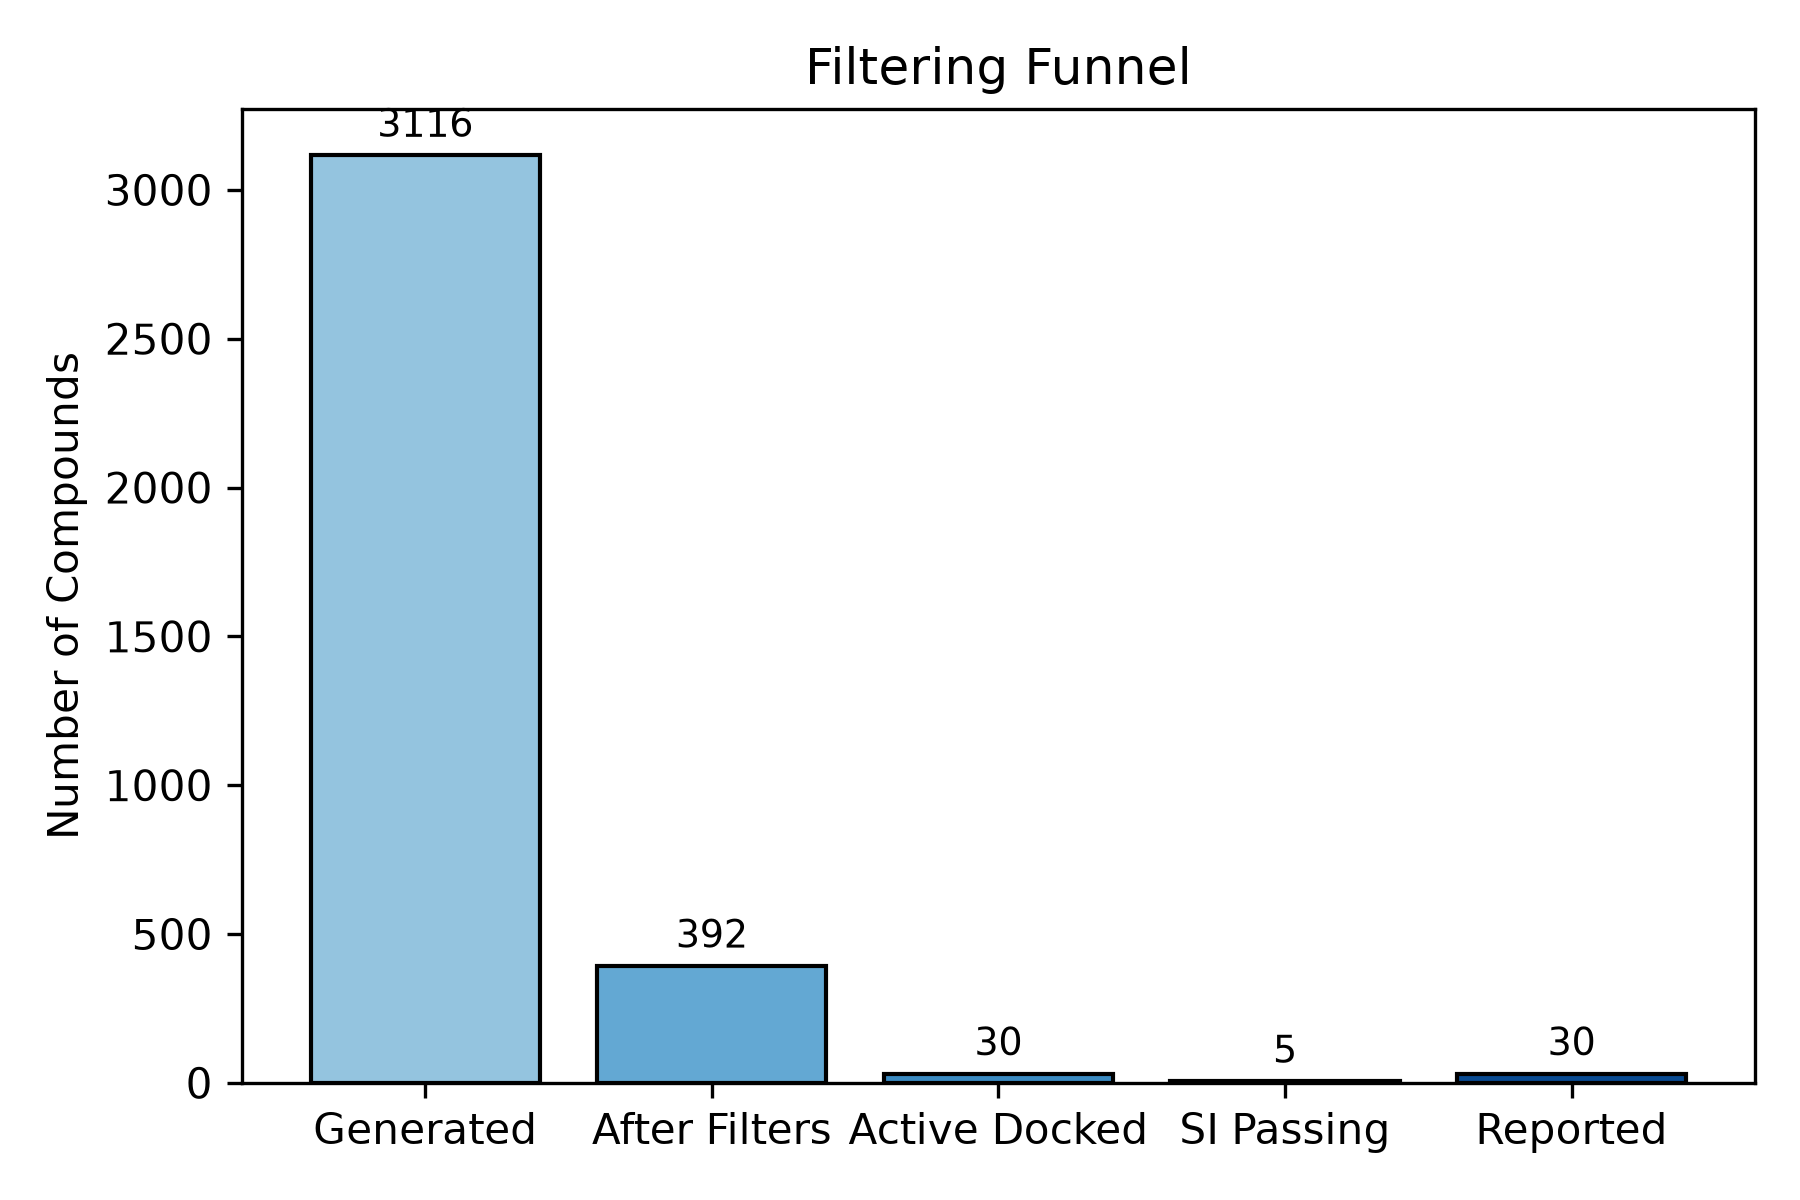
\includegraphics[width=0.65\textwidth]{output/figures/filter_funnel.png}
  \caption{Filter funnel showing compound attrition from initial library through each filtering step to the final reported set.}
  \label{fig:funnel}
\end{figure}

\section{Discussion}

\subsection{Pipeline validation}
The AutoAntibiotic v5.1.0 pipeline successfully performed a validated redocking of the native ligand ceftaroline, achieving a core RMSD of~\SI{1.251}{\angstrom} (``Validated'' badge). The consensus docking protocol across three PBP2a conformers provides robustness against conformational bias, and the mechanism-restricted selectivity profiling against two serine hydrolases reduces the risk of identifying promiscuous inhibitors.

\subsection{ALL-QU05 as a validated hit}
The top candidate ALL-QU05 satisfies the hard success criterion: it carries a ``Validated'' protocol trust badge, achieves an SI~=~2.06 (Strong tier), and forms confirmed contacts with Ser403, Lys406, and Tyr446. The compound is drug-like (QED~=~0.52, SA~=~2.13, MW~=~367.4, no PAINS, no $\beta$-lactam) and represents a genuine non-$\beta$-lactam PBP2a inhibitor candidate for experimental validation.

\subsection{Enrichment validation}
The enrichment validation passed (AUC~=~0.792, EF$_{1\%}$~=~19.25), confirming that the docking protocol enriches known PBP2a active-site binders from property-matched decoys. The benchmark used 21 known experimental PBP2a binders with assigned pIC$_{50}$ values and 150 decoys, docked against the apo (1VQQ) conformer only, consistent with standard VS enrichment practice~\cite{troczi2013}.

\subsection{Comparison with ceftaroline}
ALL-QU05's SI relative to ceftaroline (SI$_{\text{vs CEF}}$~=~1.05) indicates comparable selectivity over the clinical cephalosporin. While ceftaroline benefits from covalent inhibition of the active-site serine, ALL-QU05 achieves selective binding through non-covalent interactions alone, making it a promising starting point for optimisation.

\subsection{CES1 docking limitations}
Seven of the 20 reported candidates showed a steric clash (``CLASH (no pose)'') during CES1 docking, meaning their CES1 binding energy could not be computed and their selectivity index was unassessed. This reflects the narrower catalytic gorge of CES1 (1YAH) compared to the PBP2a active site. These compounds were retained in the report with ``Unassessed'' selectivity confidence and a provisional single-target SI computed against trypsin alone where available.

\subsection{Limitations}
The current pipeline uses rigid-receptor docking, which cannot model induced-fit effects. The static PBP2a structures may not capture the full conformational ensemble. Similarly, rigid human off-target structures may overestimate or underestimate binding. Selectivity indices are therefore approximations. No free-energy perturbation, molecular dynamics, or covalent docking was performed. All candidates should be validated experimentally through enzyme inhibition assays, SPR binding studies, and minimum inhibitory concentration (MIC) determination against MRSA strains.

\section{Conclusion}

We present a validated, reproducible consensus docking screen that identifies ALL-QU05 as a drug-like, non-$\beta$-lactam PBP2a inhibitor with confirmed contacts to Ser403, Lys406, and Tyr446 and strong selectivity over human serine hydrolases (SI~=~2.06). The AutoAntibiotic v5.1.0 pipeline, with its integrated redocking validation, consensus scoring across three conformers, and mechanism-restricted selectivity profiling, provides a robust framework for structure-based virtual screening. ALL-QU05 represents an actionable lead for experimental validation and optimisation towards a novel MRSA therapeutic.

\section*{Data availability}
All pipeline code, input data, and results are available in the AutoAntibiotic repository. The screen can be reproduced by running: \texttt{autoantibiotic --library data/screen\_library\_final.csv --count 500}. Pipeline version 5.1.0 was used for this study.

\bibliographystyle{unsrtnat}
\bibliography{references}

\end{document}
